\documentclass[dvipdfmx]{beamer}
\usepackage{tikz}
% \usepackage{gnuplot-lua-tikz}
\usepackage{empheq}
\usepackage{ulem}
\usepackage{amsmath, amsthm}
\usepackage{mathtools}
\usepackage{cases}
\usepackage{ascmac}
\usepackage{bbm}
\usepackage{capt-of}
\usetheme{Madrid}
\usefonttheme{professionalfonts} 
\setbeamertemplate{navigation symbols}{} 

% \theoremstyle{definition}
% \newtheorem{dfn}{Definition}
% \newtheorem{thm}{Theorem}
% \newtheorem{prop}{Proposition}
% \newtheorem{cor}{Corollary}

% \theoremstyle{remark}
% \newtheorem*{rem*}{Remark}

% \numberwithin{equation}{section}

%---------------------------------- mytitle---------------------------------------
\title{ポテンシャル逆問題の新たな設定と\\バブリング法による数値計算}
\date{}
\author{\textsf{守田龍平}}
\institute{京都大学大学院情報学研究科先端数理科学専攻}
%=============================================================================
%=============================================================================
\begin{document}

\begin{frame}
  \maketitle
\end{frame}

\begin{frame}{研究の概要}
  地下構造について何らかの情報を得る手段として重力探査がある.

  \begin{figure}
    \centering
    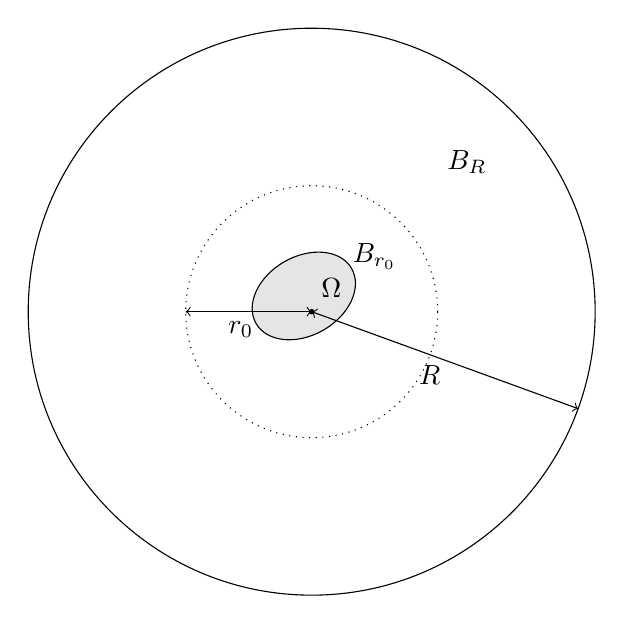
\begin{tikzpicture}
      \filldraw [fill=black!10!] (-0.1,0.2)circle[x radius=0.7,y radius=0.5,rotate=30];
      \draw(0,0.3)node[right]{$\Omega$};
      \draw(0.4,0.7)node[right]{$B_{r_0}$};
      \draw(1.6,1.9)node[right]{$B_R$};
      \draw[<->](0,0)--(-1.6,0);
      \draw[<->](0,0)--({3.6*cos(-20)},{3.6*sin(-20)});
      \draw (-0.9,0)node[below]{$r_0$};
      \draw (1.5,-0.8)node{$R$};
      \fill (0,0) circle (1pt); 
      \draw[dotted] (0,0)circle[radius=1.6];
      \draw (0,0)circle[radius=3.6];
    \end{tikzpicture}
  \end{figure}


\end{frame}

\begin{frame}{発表内容}
  \begin{enumerate}
    \item ポテンシャルの定義と性質
    \item ポテンシャル逆問題とは
    \item 数値計算の概要
    \item 数値計算例
    \item 結論
  \end{enumerate}
\end{frame}

\begin{frame}{ポテンシャルの定義と性質}
  Euclid空間$\mathbb{R}^d$の次元$d$は$2$または$3$とする.

  ある物体の密度関数$\mu(x)$に対して,$x\in\mathbb{R}^d$について
  \begin{align}\label{teigi}
    U^{\mu}(x) 
    & = \int_{\mathbb{R}^d}E(x-y)\mu(y)dy \nonumber \\ 
    & = \int_{B_{r_0}}E(x-y)\mu(y)dy \nonumber
  \end{align}
  として定め,密度関数$\mu$に対する(重力)ポテンシャルと呼ぶ.
  ポテンシャル$U^\mu$は$(\overline{B}_{r_0})^c$で調和である.

  関数$E(x)$を
  \begin{empheq}[left={E(x)=\empheqlbrace}]{alignat=2}
    & \ \ \  \frac{1}{4\pi}\frac{1}{|x|},\quad &(d=3), \nonumber \\
    & -\frac{1}{2\pi}\log{|x|},\quad &(d=2) \nonumber
  \end{empheq}
  とする.
\end{frame}


\begin{frame}{ポテンシャル逆問題とは(1/3)}
  惑星の二層モデルを考える.

  惑星の占める領域$B_R$の平均的な密度を一様に$1$とし,$\Omega\subset B_{r}$の相対的な密度を一様に$\rho$とする.
  \begin{figure}
    \centering
    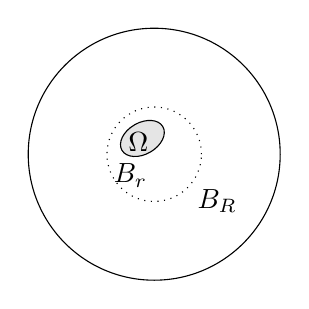
\begin{tikzpicture}
      \filldraw [fill=black!10!] (-0.15,0.2)circle[x radius=0.3,y radius=0.2,rotate=30];
      \draw(-0.2,0.15)node{$\Omega$};
      % \draw[<->](0,0)--(-0.6,0);
      % \draw[<->](0,0)--({1.6*cos(-20)},{1.6*sin(-20)});
      \draw (-0.3,0)node[below]{$B_{r}$};
      \draw (0.8,-0.6)node{$B_R$};
      % \fill (0,0) circle (1pt); 
      \draw[dotted] (0,0)circle[radius=0.6];
      \draw (0,0)circle[radius=1.6];
    \end{tikzpicture}
  \end{figure}


  このとき,$\partial B_R$上で観測するポテンシャルの密度関数$\mu_e=\mathbbm{1}_{B_R}+\rho\mathbbm{1}_{\Omega}$である.
  従って,$\partial B_R$上で観測するポテンシャル$U^{\mu_e}$は
  \begin{align*}
    U^{\mu_e}(x) = U^{\mathbbm{1}_{B_R}}(x) + \rho U^{\mathbbm{1}_\Omega}(x),\quad x\in\partial B_R
  \end{align*}
  となる.
\end{frame}

\begin{frame}{ポテンシャル逆問題とは(2/3)}
  特に,相対的な密度$\rho$を$1$とすると,
  \begin{align*}
    U^{\mathbbm{1}_\Omega}(x) = U^{\mu_e}(x) - U^{\mathbbm{1}_{B_R}}(x),\quad x\in\partial B_R
  \end{align*}
  を得る.

  右辺第1項は観測値,第2項は計算できる値だから,
  \underline{$U^{\mathbbm{1}_\Omega}$は$\Omega$の形を知らなくても$\partial B_R$上で既知である.}
  \begin{figure}
    \centering
    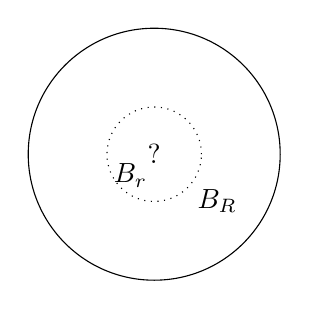
\begin{tikzpicture}
      % \filldraw [fill=black!10!] (-0.15,0.2)circle[x radius=0.3,y radius=0.2,rotate=30];
      \draw(-0,0)node{?};
      % \draw[<->](0,0)--(-0.6,0);
      % \draw[<->](0,0)--({1.6*cos(-20)},{1.6*sin(-20)});
      \draw (-0.3,0)node[below]{$B_{r}$};
      \draw (0.8,-0.6)node{$B_R$};
      % \fill (0,0) circle (1pt); 
      \draw[dotted] (0,0)circle[radius=0.6];
      \draw (0,0)circle[radius=1.6];
    \end{tikzpicture}
  \end{figure}
  ポテンシャル逆問題は,$\mu=\mathbbm{1}_{\Omega}$としたときの$\Omega$の形状を求めることに帰着される.
  以下,$\mu=\mathbbm{1}_\Omega$とする.
\end{frame}

\begin{frame}{ポテンシャル逆問題とは(3/3)}
  有界領域$\Omega\subset\mathbb{R}^d$とする.
  観測面$\partial B_R$上で重力$g$を観測し,密度関数$\mu=\mathbbm{1}_\Omega$をもつ物体の形状$\Omega$を回復する.
    \[
      \nabla U^{\mathbbm{1}_\Omega} = g \quad \mathrm{on} \quad \partial B_R \nonumber
    \]
  をみたす$\Omega$を求める.
  \begin{itembox}[c]{注目ポイント}
  現在では,原子時計によるポテンシャル$p$の直接観測の可能性があり,下段を 
  \[
    U^{\mathbbm{1}_\Omega} = p \quad \mathrm{on} \quad \partial B_R
  \]
  とした新たな問題設定を考える.
  \end{itembox}
  以下では,$\Omega\subset B_r$とする$r>0$を1つとり$r_0$とする.
\end{frame}

\begin{frame}{数値計算概要(1/2)}
  \begin{itemize}
    \item 重力観測
    \[
      \nabla U^{\mathbbm{1}_\Omega} = g \quad \mathrm{on} \quad \partial B_R. \nonumber
    \]
  
    \item ポテンシャル観測
    \[
      U^{\mathbbm{1}_\Omega} = p \quad \mathrm{on} \quad \partial B_R. \nonumber
    \]
  \end{itemize}
領域回復のアルゴリズムは次の2つのアルゴリズムから成る.
\begin{itemize}
  \item 観測点上の重力またはポテンシャルを有限個の質点で近似する \\
  Newton法もしくはLevenberg-Marquardt法
  \item 外部領域で重力またはポテンシャルが等しくなるように質量を均す \\
  Partial Mass Scattering
\end{itemize}
ポテンシャル逆問題の数値計算は主としてZidarov(1990)に倣う.

\end{frame}

\begin{frame}{数値計算概要(2/2)}
$\partial B_R$上の観測点で観測し,$B_{r_0}$に埋没している物体の形$\Omega$を回復する.
  \begin{figure}
    \centering
    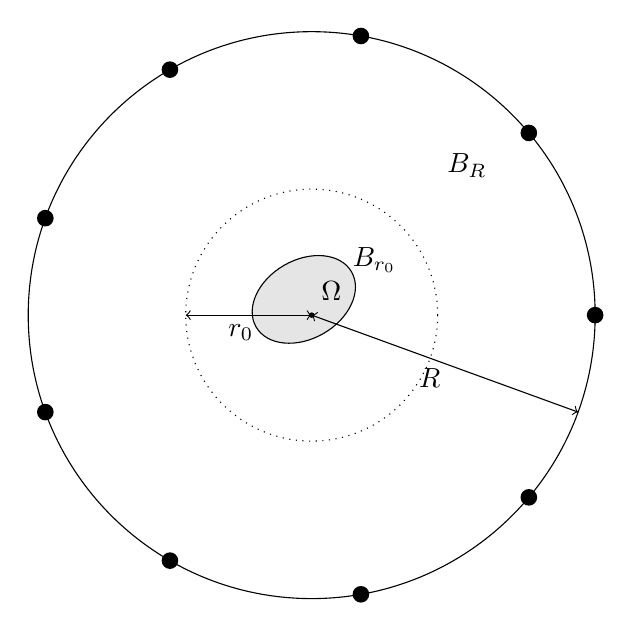
\begin{tikzpicture}
      \filldraw [fill=black!10!] (-0.1,0.2)circle[x radius=0.7,y radius=0.5,rotate=30];
      \draw(0,0.3)node[right]{$\Omega$};
      \draw(0.4,0.7)node[right]{$B_{r_0}$};
      \draw(1.6,1.9)node[right]{$B_R$};
      \draw[<->](0,0)--(-1.6,0);
      \draw[<->](0,0)--({3.6*cos(-20)},{3.6*sin(-20)});
      \draw (-0.9,0)node[below]{$r_0$};
      \draw (1.5,-0.8)node{$R$};
      \fill (0,0) circle (1pt); 
      \draw[dotted] (0,0)circle[radius=1.6];
      \draw (0,0)circle[radius=3.6];

      \fill ({3.6*cos(0)},{3.6*sin(0}) circle (3pt); 
      \fill ({3.6*cos(40)},{3.6*sin(40}) circle (3pt); 
      \fill ({3.6*cos(80)},{3.6*sin(80}) circle (3pt); 
      \fill ({3.6*cos(120)},{3.6*sin(120}) circle (3pt); 
      \fill ({3.6*cos(160)},{3.6*sin(160}) circle (3pt); 
      \fill ({3.6*cos(200)},{3.6*sin(200)}) circle (3pt); 
      \fill ({3.6*cos(240)},{3.6*sin(240}) circle (3pt); 
      \fill ({3.6*cos(280)},{3.6*sin(280}) circle (3pt); 
      \fill ({3.6*cos(320)},{3.6*sin(320}) circle (3pt); 
    \end{tikzpicture}
  \end{figure}

\end{frame}


\begin{frame}{観測した重力を有限個の質点で近似する}

  \begin{screen}
    観測点:$\{A_n\}_{n=1}^N\subset \partial B_R$,
    質点の位置:$\{X_k\}_{k=1}^K$,
    質点の質量:$\{M_k\}_{k=1}^K$ 
  \end{screen}

  $\nabla U_n^\mu=\nabla U^\mu(A_n)$と略記し,
  質点の質量分布を$\mu_K = \sum_{k=1}^K M_k\delta_{X_k}$,
  質点の系を$(X,M)=(X_1,\dots X_K,\dots ,M_1,\dots M_K)$で表す.

  コスト関数$J_G$を
  \begin{gather*}
    J_G(X, M) = \frac{1}{N}\sum_{n=1}^N(\nabla U^{\mathbbm{1}_\Omega}_n - \nabla U^{\mu_K}_n(X, M))^2,\\ 
    \quad \nabla U^{\mu_K}_n(X,M) = \frac{1}{4\pi}\sum_{k=1}^K\frac{M_k(A_n-X_k)}{|A_n-X_k|^3}
  \end{gather*}
  として定める.
\end{frame}

\begin{frame}{観測したポテンシャルを有限個の質点で近似する}
  \begin{screen}
    観測点:$\{A_n\}_{n=1}^N\subset \partial B_R$,
    質点の位置:$\{X_k\}_{k=1}^K$,
    質点の質量:$\{M_k\}_{k=1}^K$ 
  \end{screen}

  $U_n^\mu=U^\mu(A_n)$と略記し,
  質点の質量分布を$\mu_K = \sum_{k=1}^K M_k\delta_{X_k}$,
  質点の系を$(X,M)=(X_1,\dots X_K,\dots ,M_1,\dots M_K)$で表す.


  コスト関数$J_P$を
  \begin{gather*}
    J_P(X, M) = \frac{1}{N}\sum_{n=1}^N(U^{\mathbbm{1}_\Omega}_n - U^{\mu_K}_n(X,M))^2, \\
    U^{\mu_K}_n(X,M) = \frac{1}{4\pi}\sum_{k=1}^K \frac{M_k}{|A_n-X_k|}
  \end{gather*}
  として定める.
\end{frame}


\begin{frame}{Parital Mass Scattering}
  質点の系を密度$1$の物体に均す.

  領域$B_{r_0}$を幅$h$のメッシュで切り,
  質点$(X_k,M_k)$を最近傍格子点に移す.
  格子点$(i,j)$に乗っている質量を$\mu_{i,j}$で表す.
  $\Delta\mu_{ij} = \mu_{ij}-h^2 > \varepsilon$とき,
  \begin{gather*}
    \mu_{i,j}^{(1)}=h^2-\varepsilon, \\
    \mu_{i\pm 1,j}^{(1)}=\mu_{i\pm 1,j}+\frac{1}{4}(\Delta \mu_{i,j}+\varepsilon),\quad
    \mu_{i,j\pm 1}^{(1)}=\mu_{i,j\pm 1}+\frac{1}{4}(\Delta \mu_{i,j}+\varepsilon)\quad
  \end{gather*}
  として更新する.
  全ての$\Delta\mu_{i,j}$が$\varepsilon$より小さくなるまで続けることで,質量が拡散した格子点$(i,j)$については$h^2-\varepsilon\leq\mu_{i,j}\leq h^2+\varepsilon$となる.

  \begin{figure}
    \begin{tikzpicture}
      \draw [dotted,thin] (-2,-2) grid (2,2);
      \fill (0,0) circle (3pt); 
      \fill (-1,0) circle (3pt); 
      \fill (1,0) circle (3pt); 
      \fill (0,1) circle (3pt); 
      \fill (0,-1) circle (3pt); 
      \draw(0.4,0.3)node{$\mu_{i,j}$};
      \draw[->](0.2,0)--(0.8,0);
      \draw[->](0,0.2)--(0,0.8);
      \draw[->](-0.2,0)--(-0.8,0);
      \draw[->](0,-0.2)--(0,-0.8);
    \end{tikzpicture}
  \end{figure}

\end{frame}

\begin{frame}{数値計算 目標の確認}
  原点中心半径$r_0=2$の円$B_{r_0}$に物体が含まれていることは事前情報として与えられているとき,
  観測半径$R$を変えたときの影響を調査する.
  \begin{figure}
    \centering
    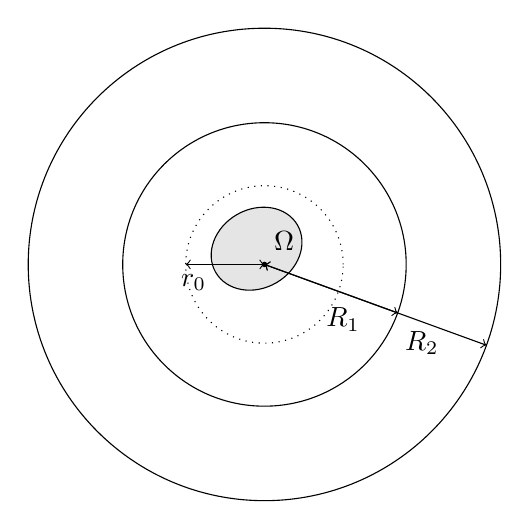
\begin{tikzpicture}
      \filldraw [fill=black!10!] (-0.1,0.2)circle[x radius=0.6,y radius=0.5,rotate=30];
      \draw(0,0.3)node[right]{$\Omega$};
      \draw[<->](0,0)--(-1.0,0);
      \draw (-0.9,0)node[below]{$r_0$};
      \fill (0,0) circle (1pt); 
      \draw[dotted] (0,0)circle[radius=1.0];
      \draw (0,0)circle[radius=1.8];
      \draw[<->](0,0)--({1.8*cos(-20)},{1.8*sin(-20)});
      \draw (1,-0.7)node{$R_1$};
      \pause 
      \draw[<->](0,0)--({3.0*cos(-20)},{3.0*sin(-20)});
      \draw (2,-1)node{$R_2$};
      \draw (0,0)circle[radius=3.0];

    \end{tikzpicture}
  \end{figure}
\end{frame}

\begin{frame}{数値計算 最適化アルゴリズムの設定}
最適化アルゴリズムのステップ数を$l$とし,$l$ステップ目の各質点を$(X_k^{(l)}, M_k^{(l)})$とする.
  \begin{itembox}{観測値と初期値}
    $\partial B_R$上等間隔に$N$個の観測点$\{A_n\}_{n=1}^N$をとる.
    観測器の精度は小数点以下$8$桁で固定とする.

    $\partial B_{r_0}$上等間隔に$K$個の初期地点$\{X_k^{(0)}\}_{k=1}^K$をとり,
    各質点の質量は $M_k^{(0)} = \pi r_0^2/K$ とする.
  \end{itembox}
  
  \begin{itembox}{停止条件}
    質点$(X_k, M_K)$の位置を$X_k=(x_k, y_k)$とし,
    \[
      |x_k^{(l+1)}-x_k^{(l)}| < 10^{-2},\quad
      |y_k^{(l+1)}-y_k^{(l)}| < 10^{-2},\quad
      |M_k^{(l+1)}-M_k^{(l)}| < 10^{-2}
    \]
    を全ての$k$について満たすとき,最適化アルゴリズムを停止する.
  \end{itembox}
\end{frame}



\begin{frame}{数値計算 Partial Mass Scatteringの設定}
  格子点$(i,j)$に乗っている質量を$\mu_{i,j}$で表す.
  $\Delta\mu_{ij} = \mu_{ij}-h^2 > \varepsilon$とき,
  \[
    \mu_{i,j}=h^2-\varepsilon
  \]
  で更新する.
  メッシュ幅$h$は$10^{-2}$とし,パラメータ$\varepsilon$は$10^{-6}$とした.
  \begin{figure}
    \begin{tikzpicture}
      \draw [dotted,thin] (-2,-2) grid (2,2);
      \fill (0,0) circle (3pt); 
      \fill (-1,0) circle (3pt); 
      \fill (1,0) circle (3pt); 
      \fill (0,1) circle (3pt); 
      \fill (0,-1) circle (3pt); 
      \draw(0.4,0.3)node{$\mu_{i,j}$};
      \draw[->](0.2,0)--(0.8,0);
      \draw[->](0,0.2)--(0,0.8);
      \draw[->](-0.2,0)--(-0.8,0);
      \draw[->](0,-0.2)--(0,-0.8);
    \end{tikzpicture}
  \end{figure}
\end{frame}

% \begin{frame}{円板の回復}
  % 原点中心半径$1$の円板の回復を試みる.

  % 質点の数$K=1$,観測点$N=3$とし,観測半径$R$を変えてその影響について数値計算する.
  % 最適化にはNewton法を用いた.
  % コスト関数$J_P, J_G$を$0$とする$(X_1,M_1)$が存在し,いずれの場合も$X_1=0, M_1=\pi$に限られている.

  % \begin{figure}
    % \centering
    % \begin{tikzpicture}
      % \filldraw [fill=black!10!] (0,0) circle [radius=0.5];
      % \fill (0,0) circle (1pt); 
      % \draw[dotted] (0,0)circle[radius=1];
      % \draw[<->](0,0)--(-1,0);
      % \draw[<->](0,0)--({2*cos(-20)},{2*sin(-20)});
      % \draw(1.5,0)node[below]{$R$};
      % \draw(-0.7,0)node[above]{$r_0$};
      % \draw (0,0)circle[radius=2];
      % \fill (2,0) circle (3pt); 
      % \fill ({2*cos(0)},{2*sin(0}) circle (3pt); 
      % \fill ({2*cos(120)},{2*sin(120}) circle (3pt); 
      % \fill ({2*cos(240)},{2*sin(240}) circle (3pt); 
    % \end{tikzpicture}
  % \end{figure}

% \end{frame}



\begin{frame}{正三角形の回復}
  原点中心で,重心から各頂点への距離が1の正三角形の回復を試みる.
  最適化にはLevenberg-Marquardt法を用いた.

  \begin{figure}
    \centering
    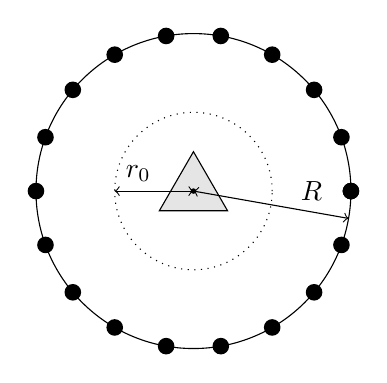
\begin{tikzpicture}
      \filldraw[fill=black!10!] ({-0.25*sqrt(3)},-0.25) -- ++(0:{0.5*sqrt(3)}) -- ++(120:{0.5*sqrt(3)}) -- cycle;
      \fill (0,0) circle (1pt); 
      \draw[dotted] (0,0)circle[radius=1];
      \draw[<->](0,0)--(-1,0);
      \draw[<->](0,0)--({2*cos(-10)},{2*sin(-10)});
      \draw(1.5,0)node{$R$};
      \draw(-0.7,0)node[above]{$r_0$};
      \draw (0,0)circle[radius=2];
      \fill (2,0) circle (3pt); 
      \fill ({2*cos(0)},{2*sin(0}) circle (3pt); 
      \fill ({2*cos(20)},{2*sin(20}) circle (3pt); 
      \fill ({2*cos(40)},{2*sin(40}) circle (3pt); 
      \fill ({2*cos(60)},{2*sin(60}) circle (3pt); 
      \fill ({2*cos(80)},{2*sin(80}) circle (3pt); 
      \fill ({2*cos(100)},{2*sin(100}) circle (3pt); 
      \fill ({2*cos(120)},{2*sin(120}) circle (3pt); 
      \fill ({2*cos(140)},{2*sin(140}) circle (3pt); 
      \fill ({2*cos(160)},{2*sin(160}) circle (3pt); 
      \fill ({2*cos(180)},{2*sin(180}) circle (3pt); 
      \fill ({2*cos(200)},{2*sin(200}) circle (3pt); 
      \fill ({2*cos(220)},{2*sin(220}) circle (3pt); 
      \fill ({2*cos(240)},{2*sin(240}) circle (3pt); 
      \fill ({2*cos(260)},{2*sin(260}) circle (3pt); 
      \fill ({2*cos(280)},{2*sin(280}) circle (3pt); 
      \fill ({2*cos(300)},{2*sin(300}) circle (3pt); 
      \fill ({2*cos(320)},{2*sin(320}) circle (3pt); 
      \fill ({2*cos(340)},{2*sin(340}) circle (3pt); 
    \end{tikzpicture}
  \end{figure}

\end{frame}

\begin{frame}{正三角形の回復 重力観測}
  質点の数$K=30$,観測点数$N=90$とする.
  \begin{columns}
    \centering
    \begin{column}[b]{0.48\columnwidth}
      \centering
      \includegraphics[width=4.5cm]{fig/triangle.png}
      \captionof{figure}{答え}
    \end{column}
    \hspace{-3cm}
    \begin{column}[b]{0.48\columnwidth}
      \centering
      \includegraphics[width=4.5cm]{fig/GR6N90K30E4.png}
      \captionof{figure}{観測半径$R=6$}
    \end{column}
  \end{columns}

  % \begin{columns}
    % \centering
    % \begin{column}[b]{0.48\columnwidth}
      % \centering
      % \includegraphics[width=4.5cm]{fig/triangle.png}
      % \captionof{figure}{答え}
    % \end{column}
    % \hspace{-3cm}
    % \begin{column}[b]{0.48\columnwidth}
      % \centering
      % \includegraphics[width=4.5cm]{fig/GR6N90K30E4.png}
      % \captionof{figure}{観測半径$R=60$}
    % \end{column}
  % \end{columns}

\end{frame}

\begin{frame}{正三角形の回復 ポテンシャル観測}
  質点の数$K=30$,観測点数$N=90$とする.
  \begin{columns}
    \centering
    \begin{column}[b]{0.48\columnwidth}
      \centering
      \includegraphics[width=4.5cm]{fig/triangle.png}
      \captionof{figure}{答え}
    \end{column}
    \hspace{-3cm}
    \begin{column}[b]{0.48\columnwidth}
      \centering
      \includegraphics[width=4.5cm]{fig/PR6N90K30E4.png}
      \captionof{figure}{観測半径$R=6$}
    \end{column}
  \end{columns}

  \begin{columns}
    \centering
    \begin{column}[b]{0.48\columnwidth}
      \centering
      \includegraphics[width=4.5cm]{fig/triangle.png}
      \captionof{figure}{答え}
    \end{column}
    \hspace{-3cm}
    \begin{column}[b]{0.48\columnwidth}
      \centering
      \includegraphics[width=4.5cm]{fig/PR60N90K30E4.png}
      \captionof{figure}{観測半径$R=60$}
    \end{column}
  \end{columns}


\end{frame}


\begin{frame}{結論}

  ポテンシャル逆問題において,境界でポテンシャルを既知とする問題設定を行い,重力を既知とする場合と比較して数値計算を行った.

  \begin{itemize}

    \item 正三角形の回復

    観測半径$R$を増大させた影響をみた.
    ポテンシャル観測による物体の回復の方が細部を回復する可能性が高いことを示唆している.
  \end{itemize}

\end{frame}

\begin{frame}{参考文献}
  \begin{thebibliography}{99}
    \bibitem{An}
    G.Anger, 
    \textit{Inverse Problems in Differential Equations},
    Plenum Press,
    1990.
  
    \bibitem{Yu}
    萩原幸男,
    『測地学入門』,
    東京大学出版会,
    1982.
  
    \bibitem{Is}
    V.Isakov,
    \textit{Inverse Source Problems},
    American Mathematical Society,
    1990.
  
    \bibitem{Kr}
    R.Kress,
    \textit{Numerical Analysis},
    Springer,
    1998.
  
    \bibitem{No}
    野崎京三,
    『原子時計をセンサーとした重力ポテンシャル計の可能性』,
    応用地質技術年報,30号(2011),65-71.
  
    \bibitem{Sa}
    佐々木晶,
    『惑星内部構造』,
    地震,61巻特集号(2009),285-296.
  
  
    \bibitem{Za}
    L.Zalcman,
    Some Inverse Problems of Potential Theory,
    \textit{Contemporary Mathematics}, Vol.63(1987), 337-339.
  
    \bibitem{Zi} 
    D.Zidarov, 
    \textit{Inverse Gravimetric Problem in Geoprospecting and Geodesy},
    Elsevier,
    1990.
  \end{thebibliography}

\end{frame}

\end{document}
